\documentclass[a4paper]{article}
% standard packages
\usepackage{amssymb}
\usepackage{euscript}
\usepackage{eurosym}
\usepackage{graphicx}
\graphicspath{{img/}}
\usepackage{color}
\usepackage{epsfig}
\usepackage{fullpage}
\usepackage[colorlinks=true]{hyperref}
\usepackage{titling}

% title style
\pretitle{\noindent\LARGE}
\posttitle{\\[1ex]}
\preauthor{\large}
\postauthor{,}
\predate{\large(}
\postdate{)}
\date{last update: \today}

% large page size
\oddsidemargin -1cm
\topmargin -1cm
\textwidth 18cm
\textheight 27cm
\pagestyle{empty}


% PDF figure (floating)
\newcommand{\image}[3]{
\begin{figure}[#1]
\begin{center}
\caption{\small#3}
\includegraphics{img_#2.pdf}
\label{image:#2}
\end{center}
\end{figure}
}

% simple image
\newcommand\simpleimage[3][\linewidth]{
\smallskip\begin{center}\vbox{\noindent
\includegraphics[width=#1]{#2}\\%
\parbox{#1}{\it#3}}\end{center}
\medskip}

%\newcommand\simpleimage[3][\linewidth]{
%\smallskip\vbox{\noindent
%\includegraphics[width=#1]{#2}\\%
%\it#3}
%\medskip}


% companies
\def\SchaefferAG{\href{https://www.schaeffer-ag.de/en/}{Schaeffer-AG}}
\def\MultiCB{\href{https://portal.multi-circuit-boards.eu}{Multi-CB}}
\def\BlueFors{\href{https://www.bluefors.com/}{BlueFors}}

\def\Ohmite{\href{https://www.ohmite.com}{Ohmite}}
\def\Firmetal{\href{http://www.firmetal.com}{Firmetal}}
\def\Bruker{\href{https://www.bruker.com}{Brucker}}

% use this to refer to Farnell and RS numbers:
\def\FarnellN#1{\href{https://fi.farnell.com/#1}{Farnell:#1}}
\def\RSN#1{\href{https://fi.rsdelivers.com/productlist/search?query=#1}{RS:#1}}

% products:
\def\OhmiteOFOD{\href{https://www.ohmite.com/assets/docs/res_od_of_oa.pdf}{Ohmite OF/OD series}}

% Supplementary materials on github <report> <file>
\def\GitFile#1#2{\href{https://github.com/slazav/he3notes/raw/master/#1/#2}{#1/#2}}

% Supplementary materials on my users.aalt.fi page
\def\WWWFile#1{\href{https://users.aalto.fi/~zavyalv1/#1}{#1}}


%progams
\def\MagnettiProg{\href{https://github.com/slazav/magneetti}{\tt magnetti}}



\title{BNC clamps}
\author{V.Zavjalov}

\twocolumn
\begin{document}
\maketitle

In CW NMR experiments with compensated signal unstable contact in BNC
connectors is a problem. Unfortunately, most of usual devices use such
connectors for signal lines. There are a few ways how one can deal with
this problem. In Dmitriev's group in Moscow all important connectors have
been replaced to TNC (a threaded version of the BNC). This needs
disassembling of devices and not always possible. In ROTA group in
Helsinki clamps have been used to attach BNC-to-SMA converters to all
connectors.

\simpleimage{img/clamp_rota.jpg}{ROTA clamp}

I am using similar clamps as in ROTA but simpler and cheaper. Clamps have
been ordered in \SchaefferAG{} company. Price was 332\euro{} for 20
aluminum clamps (two parts each). Aluminum is a bit too soft, one should
try thicker design or different metal. But clamps work pretty well.

\noindent Clamp drawing, FPD files for production:\\
\WWWFile{notes/2018-bncclamps/fpd\_v1.zip}

\begin{center}
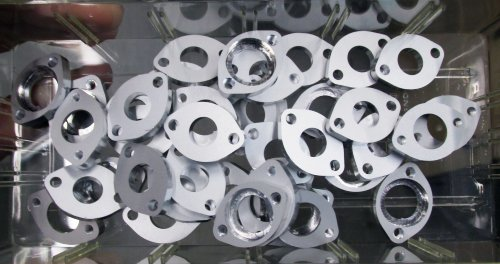
\includegraphics[width=\linewidth]{img/clamp1.jpg}
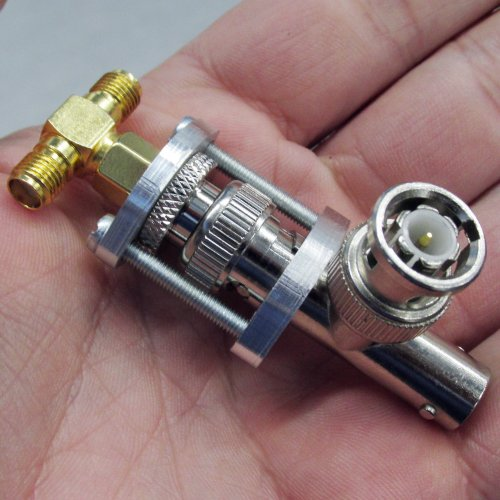
\includegraphics[width=\linewidth]{img/clamp2.jpg}
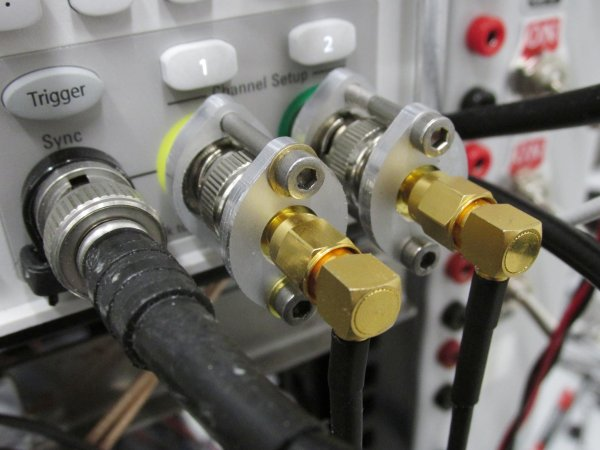
\includegraphics[width=\linewidth]{img/clamp3.jpg}
\end{center}

\end{document}






